%
\hsection{\crowsFoot{M}{M1}{N}{MM}}%
\label{sec:rm:mn}%
%
\begin{figure}%
\centering%
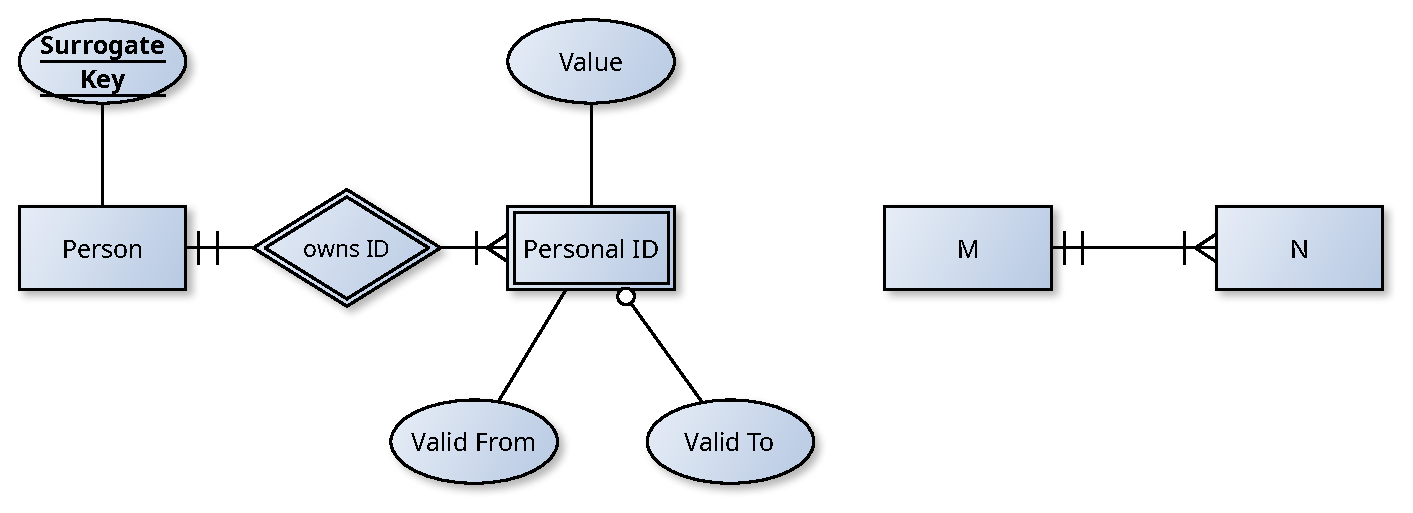
\includegraphics[width=0.9\linewidth]{\currentDir/MN}%
\caption{We encountered the \crowsFoot{M}{M1}{N}{MM} relationship pattern in \cref{fig:erdPerson4}.}%
\label{fig:rm:mn}%
\end{figure}%
%
\gitLoadAndExecSQL{MN_tables}{}{conceptualToRelational}{MN_tables.sql}{relationships}{}{}%
\listingSQLandOutput{MN_tables}{MN_tables.sql}{%
The realization of a \crowsFoot{M}{M1}{N}{MM} conceptual relationship.%
}{}%
\gitLoadAndExecSQL{MN_insert_and_select}{}{conceptualToRelational}{MN_insert_and_select.sql}{relationships}{}{}%
\listingSQLandOutput{MN_insert_and_select}{MN_insert_and_select.sql}{%
Inserting into and selecting data from the realization of an \crowsFoot{M}{M1}{N}{MM} conceptual relationship given in \cref{lst:MN_tables}.%
}{}%
%
\gitExec{cdtrmTableM}{\databasesCodeRepo}{conceptualToRelational}{../_scripts_/db_table_to_latex_table.sh relationships m mid;fknid;x}%
\gitExec{cdtrmTableN}{\databasesCodeRepo}{conceptualToRelational}{../_scripts_/db_table_to_latex_table.sh relationships n nid;fkmid;y}%
%
\begin{figure}%
\centering%
\floatSep%
\input{\gitFile{cdtrmTableM}}%
\floatSep%
\input{\gitFile{cdtrmTableN}}%
\floatSep%
\caption{The contents of the the two tables in the implementation of the \crowsFoot{M}{M1}{N}{MM} conceptual relationship after executing \cref{lst:MN_insert_and_select}.}%
\label{fig:rm:mn:tables}%
\end{figure}%
%
\gitLoadAndExecSQL{MN_insert_error_1}{}{conceptualToRelational}{MN_insert_error_1.sql}{relationships}{}{}%
\listingSQLandOutput{MN_insert_error_1}{MN_insert_error_1.sql}{%
Trying to create a row into table~\sqlil{m} that is not related to any row in table~\sqlil{n} is not possible.%
}{}%
%
\gitLoadAndExecSQL{MN_insert_error_2}{}{conceptualToRelational}{MN_insert_error_2.sql}{relationships}{}{}%
\listingSQLandOutput{MN_insert_error_2}{MN_insert_error_2.sql}{%
Trying to create a row into table~\sqlil{n} that is not related to any row in table~\sqlil{m} is not possible.%
}{}%
%
\gitLoadAndExecSQL{MN_insert_error_3}{}{conceptualToRelational}{MN_insert_error_3.sql}{relationships}{}{}%
\listingSQLandOutput{MN_insert_error_3}{MN_insert_error_3.sql}{%
Trying to create a row in table~\sqlil{m} that references a row in table~\sqlil{n} which is referencing another row in table~\sqlil{m} is not possible.%
}{}%
%
\gitLoadAndExecSQL{MN_insert_error_4}{}{conceptualToRelational}{MN_insert_error_4.sql}{relationships}{}{}%
\listingSQLandOutput{MN_insert_error_4}{MN_insert_error_4.sql}{%
Trying the same thing as in \cref{lst:MN_insert_error_3}, but this time also attempting to re-adjusting the row in~\sqlil{n} with an~\sqlil{UPDATE} instruction to make reference the new row in table~\sqlil{m}, is also not possible.%
}{}%
%
\gitLoadAndExecSQL{MN_insert_error_5}{}{conceptualToRelational}{MN_insert_error_5.sql}{relationships}{}{}%
\listingSQLandOutput{MN_insert_error_5}{MN_insert_error_5.sql}{%
Changing a row in table~\sqlil{n} that references a row in table~\sqlil{m} to now reference another row in table~\sqlil{m} is not possible.
}{}%
%
We have the two entity types~M and~N.
Each entity of type~M must be linked to at least one entity of type~N, but can also be linked to many of them.
Each entity of type~N is connected to exactly one entity of type~M.

We encountered this relationship pattern in \cref{fig:erdPerson4}, when we tried to model the relationship between entities of type~\emph{Person} and~\emph{Personal~ID}.
Each person must have at least one personal~ID.
Each personal~ID belongs to exactly one person.
This is illustrated in \cref{fig:rm:mn}.

Implementing the referential integrity of this relationship pattern in \sql\ is a bit complicated but doable.
I did struggle with the \crowsFoot{G}{O1}{H}{MM} relationship pattern back in \dref{sec:rm:gh}, but in the end we figured it out.
A very similar pattern can be implemented now.
We only have one more constraint, namely the one that enforces that all entities of type~N are linked to one entity of type~M each.
And this additional constraint is the same that we used back then, just \inQuotes{the other way around.}
Writing down the table structures and constraints as shown in \cref{lst:MN_tables} can thus be understood once we comprehend \cref{lst:GH_tables} from back in \cref{sec:rm:gh}.
Well, almost.

We create a table~\sqlil{m} for the entities of type~M in \cref{lst:MN_tables}.
It has primary key~\sqlil{mid} and the additional example data column~\sqlil{x}.
This also needs an attribute~\sqlil{fknid} that will later be used to reference one row in table~\sqlil{n}.
Since each entity of type~M must be linked to at least one entity of type~N, this column will be~\sqlil{NOT NULL}.
Since each entity of type~N must be linked to exactly one entity of type~M (and not more than one), we also mark the column as~\sqlil{UNIQUE}.

Now we create the table~\sqlil{n} for storing entities of type~N.
The primary key be~\sqlil{nid} and the additional example data column is~\sqlil{y}.
Since each row in~\sqlil{n} must be related to exactly one row in~\sqlil{m}, we also add a column~\sqlil{fkmid} to this table.
It \sqlil{REFERENCES} the primary key~\sqlil{mid} of table~\sqlil{m}.
The difference between \cref{lst:MN_tables} and \cref{lst:GH_tables} is that now \sqlil{fkmid} of table~\sqlil{n} is \sqlil{NOT NULL}, whereas the foreign key~\sqlil{fkgid} for table~\sqlil{h} could be~\sqlil{NULL}.
This is because every entity of type~N must be related to an entity of type~M, whereas back in \cref{sec:rm:gh}, each entity of type~H could be related to one or zero entities of type~G.
Apart from this difference, we now add the constraint \sqlil{m_fknid_mid_fk} which works exactly as \sqlil{g_fkhid_gid_fk} in \cref{lst:GH_tables}.

It turns out that this single added \sqlil{NOT NULL} constraint imposed on column~\sqlil{fkmid} of table~\sqlil{n} makes inserting data much harder.
The \inQuotes{G~end} of the relationship in \cref{sec:rm:gh} was an~\inQuotes{optionally one}.
Once we had created the tables and constraints, we could begin storing data by \emph{first} populating the table for the entities of type~H.
Then we could take of creating the records for the table for the entities of type~G and fix the referential integrity.

Regardless of how we look at it, we do not have such luck this time:
Each entity of type~N \emph{must} be linked to exactly one existing entity of type~M.
Each entity of type~M \emph{must} be linked to at least one existing entity of type~N.
This is a much worse problem, because we need to know the primary key~\sqlil{nid} of a row in table~\sqlil{n} in order to create a new row in table~\sqlil{m} and we need to know the primary key~\sqlil{mid} of a row in table~\sqlil{m} to create a new row in table~\sqlil{n}.

It is clear that we will have to use \pglspl{CTE} to approach this problem.
The only solution I could find for this problem is based on the following idea:
We need to, somehow, be able to get the value of the primary key that would be used when we create a new row in~\sqlil{m} \emph{before} creating this row.
If we know the primary key value, then we can use its value as \sqlil{fkmid} when inserting a row into table~\sqlil{n} and get the primary key of that row.
Then we use this primary key as \sqlil{fknid} and actually insert the row into table~\sqlil{m}.

This can be done if we generate the primary key for table~\sqlil{m} more explicitly than before.
So far, we would write something like \sqlil{mid INT GENERATED BY DEFAULT AS IDENTITY PRIMARY KEY}.
This means that the column is a primary key is of type~\sqlil{INT}.
It is \sqlil{GENERATED BY DEFAULT}, which means that its values or generated \emph{unless specified}~\cite{PGDG:PD:GC}.
Thus, when inserting rows into the table, we could specify a value for~\sqlil{mid}, which is then used, or we do not specify a value, in which case one will be generated for us automatically.
The \sqlil{AS IDENTITY} means that, when a value is generated, it is taken from an implicit sequence~\cite{PGDG:PD:IC}.

Instead of using an implicit sequence without name, we also create a sequence using the command~\sqlil{CREATE SEQUENCE}\sqlIdx{CREATE!SEQUENCE}~\cite{PGDG:PD:CS}.
We create a sequence~\sqlil{sqmid} to generate the primary keys for the table~\sqlil{m} in \cref{lst:MN_tables} by writing~\sqlil{CREATE SEQUENCE sqmid AS INT;}\sqlIdx{CREATE!SEQUENCE}.
Such sequences will always be strictly increasing.
The next value of \sqlil{sqmid} would be obtained atomically by~\sqlil{NEXTVAL('sqmid')}\sqlIdx{NEXTVAL}~\cite{PGDG:PD:SMF}.
We now define the primary key of table~\sqlil{m} as \sqlil{mid INT DEFAULT NEXTVAL('sqmid') PRIMARY KEY}\sqlIdx{NEXTVAL}.
This definition says that the value of the primary key~\sqlil{mid} \emph{can} be provided when creating rows in~\sqlil{m}.
If it is \emph{not} provided, then a~\sqlilIdx{DEFAULT} value will be used~\cite{PGDG:PD:DV2}.
This default value is computed by evaluating the expression~\sqlil{NEXTVAL('sqmid')}\sqlIdx{NEXTVAL}.
It will be the ever-increasing output of the sequence~\sqlil{sqmid}.%
%
\begin{sloppypar}%
From a mechanical point of view, this works more or less like \sqlil{mid INT GENERATED BY DEFAULT AS}\linebreak[3]\sqlil{IDENTITY PRIMARY KEY}.
The difference is that we now can also generate valid values for~\sqlil{mid} without creating rows in~\sqlil{m}.
Of course we can use \sqlil{NEXTVAL('sqmid')}\sqlIdx{NEXTVAL} in any \sql\ query, \sqlil{SELECT}, \sqlil{INSERT}, \sqlil{UPDATE} -- whatever we want.
And whenever \sqlil{NEXTVAL('sqmid')}\sqlIdx{NEXTVAL} is invoked, it will step the sequence~\sqlil{sqmid}.
It will never return the same value~(unless you evaluate it $2^{64}$~times).
This means that we can generate a valid primary key value for table~\sqlil{m}, then insert a row into table~\sqlil{n} using this value as foreign key, and then insert a row into table~\sqlil{m} actually using it as primary key.%
\end{sloppypar}%
%
\begin{sloppypar}%
In \cref{lst:MN_insert_and_select}, we thus insert a pair of rows into tables~\sqlil{m} and~\sqlil{n} as follows:
First, we generate the primary key for the row that we want to insert into table~\sqlil{m} as \pgls{CTE} that just invokes \sqlil{NEXTVAL('sqmid')} and remembers the result, i.e., \sqlil{m_id AS (SELECT NEXTVAL('sqmid') AS new_mid)}.
Then we insert a row into table~\sqlil{n}, also as \pgls{CTE}, by doing \sqlil{new_n AS (INSERT INTO n (y, fkmid) SELECT 'AB', new_mid FROM m_id RETURNING nid, fkmid)}.
This \pgls{CTE} returns the primary key~\sqlil{nid} of the new row in table~\sqlil{n} as well as the previously generated primary key~\sqlil{new_mid} for the row that we will insert into table~\sqlil{m}~(as \sqlil{fkmid}).
We use both values in to finally actually insert the row into table~\sqlil{m} by calling \sqlil{INSERT INTO m (mid, x, fknid) SELECT fkmid, '123', nid FROM new_n;}.%
\end{sloppypar}%
%
After this, if we want to append  another row to table~\sqlil{n} and link it to the now existing row in table~\sqlil{m}, we can do this more easily via~\sqlil{INSERT INTO n (y, fkmid) VALUES ('CD', 1);}.
The creation of new rows for table~\sqlil{m}, however, requires us to have the two \pglspl{CTE}.
The contents of the tables~\sqlil{m} and~\sqlil{n} after inserting the data are shown in \cref{fig:rm:mn:tables}.
Reassembling the data from both tables can be achieved with a single~\sqlil{INNER JOIN}, as illustrated at the bottom of \cref{lst:MN_insert_and_select}.

This solution requires several \postgresql-specific techniques, such as \sqlilIdx{RETURNING}, \sqlilIdx{NEXTVAL}, and the creation of sequences.
Other \pglspl{dbms} certainly have similar or slightly different extensions to the \sql\ standard that allow us to do similar things.
In \cref{lst:MN_insert_error_1,exec:MN_insert_error_1,lst:MN_insert_error_2,exec:MN_insert_error_2,lst:MN_insert_error_3,exec:MN_insert_error_3,lst:MN_insert_error_4,exec:MN_insert_error_4,lst:MN_insert_error_5,exec:MN_insert_error_5} we perform similar sanity tests as back in \cref{sec:rm:gh}.
We confirm that our constraints protect the referential integrity of the data.%
%
\FloatBarrier%
\endhsection%
%
